\chapter{Continuous Micromagnetics}
\label{sec:cont-micromag}

In \thisref{sec:comp-meth} we give an introduction to the theory of micromagnetics including a statement of the equations to be solved.
Micromagnetics is a semi-classical (\ie quantum mechanical effects are approximated using classical techniques), continuum (\ie the fields involved are assumed to be ``smooth'') theory of ferromagnetism.
It is widely used to describe the behaviour of ferromagnetic materials on scales above those accessible using quantum mechanical approaches such as density functional theory.


??Ds talk about physical origins of m a bit?

\section{Definitions}
We define $\Mv(\xv,t)$ to be a vector field representing the expectation value of the magnetisation per unit volume averaged over a number of unit cells \cite{Aharoni1996}.
The length of $\Mv(\xv,t)$ is fixed and given by the saturation magnetisation $M_s$, a material parameter.
We define $\Hv(\xv,t)$ to be the magnetic field.
These quantities are related to the magnetic flux density $\Bv(\xv,t)$ (in units of Tesla) by
\begin{equation}
  \label{eq:37}
  \Bv(\xv,t) = \mu_0 \left( \Hv(\xv,t) + \Mv(\xv,t) \right),
\end{equation}
% \cite{Gilbert2004} says that this magnetisation is different - averaged over all material rather than over a few cells...
where $\mu_0$ is the magnetic constant (or permeability of free space).

\begin{figure}
  \center
  \begin{tikzpicture}
    \draw[line width=0.5mm,fill=paleblue,draw=solidblue] (0,0) ellipse (3cm and 1.5cm);
    \draw (0,0) node {\Large{$\magd$}};
    \draw (2.8,0.8) node[anchor=west] {\Large{$\boundd$}};
    \draw (-6,1) node[anchor=north] {\Large{$\extd$}};
  \end{tikzpicture}
  \caption{The domain labels used: $\magd$ is the magnetic material, $\boundd$ is the boundary and $\extd$ is the (infinite) external region.} \label{fig:domain_labels}
\end{figure}

Our labelling of the domains is shown in \cref{fig:domain_labels}.
We call the region of magnetic material $\magd$, it's boundary $\boundd$ and the external domain $\extd$.

When working with equations in dimensional form we always use S.I. units.
In general we will not make dependencies on $\xv$ and $t$ explicit.




\section{The energy of a magnetic body}
\label{sec:energy-magnetic-body}

A number of energy terms are included in standard micromagnetic models: the magnetostatic self field, the exchange energy and the magnetocrystalline anisotropy energy.
Also important is the external applied field due to magnetic bodies or electrical currents outside the modelled region.
We begin by providing a description of each of these energies.
Other effects which are sometimes important include temperature (thermal effects) and magnetostriction (the change in magnetic behaviour due to stretching or compressing the magnet).

The energy due to an external applied field (sometimes called the Zeeman energy) is 
\begin{equation}
  \label{eq:42}
  \Eapp = - \mu_0 \int_{\magd} \Mv \cdot \Happ \d \magd.
\end{equation}

By inverting \cref{eq:42} we can obtain an ``effective field'' $\Hv$ for any energy term $E$:
\begin{equation}
  \Hv = \dfrac{-1}{\mu_0V_{\magd}} \dfrac{\delta E}{\delta \Mv},
  \label{eq:62}
\end{equation}
where $\delta$ indicates a variational derivative and $V_{\magd}$ is the volume of the magnetic domain.
This effective field acts exactly like a real field in calculations of the magnetisation dynamics and represents the effects of the corresponding energy term.


%% Energy and field expressions below are taken from Matteo Franchin's thesis \cite{Franchin2009}.\footnote{Note that due to the variety in unit systems, definitions of magnetisation and other choices it can be difficult to compare energy/effective field equations from different authors, in particular the location of factors of $\mu_0$.}

\subsection{Exchange energy}

In a ferromagnetic material neighbouring magnetic moments prefer to align parallel to each other due to quantum mechanical effects. 
This can be approximated by a classical expression for exchange energy \cite{Aharoni1996} as
\begin{equation}
  \label{eq:39}
  \Eex =  \frac{\Exchc}{M_s^2} \int_{\magd} (\nabla M_x)^2  + (\nabla M_y)^2  + (\nabla M_z)^2 \d \magd,
\end{equation}
where $\Exchc$ is the material dependent exchange constant representing the strength of the exchange coupling.

We write the vector Laplacian as $\lap \Mv = (\lap M_x,\lap M_y, \lap M_z )$. 
Then the exchange effective field is given by
\begin{equation}
  \label{eq:Hex}
  \Hex = \frac{2 \Exchc}{ \mu_0 M_s} \lap \Mv.
\end{equation}


\subsection{Magnetostatic energy}
\label{sec:magnetostatic-field}

Magnetic materials generate a magnetic field, which in turn affects the magnetic material emitting the field. 
This type of field is also known as the demagnetising field as it tends to oppose the magnetisation of the body. 
The magnetostatic field, $\Hms$, can be written in two ways: an integral form or a differential (potential) form. 
% These methods are discussed in \cref{sec:magstat-field-calc-inte} and \ref{sec:magstat-field-calc-pote} respectively.

The integral form of the magnetostatic field at a point $\xv \in \real^3$ due to the magnetic body $\magd$ with boundary $\boundd$ can be given in terms of magnetisation $\Mv$ by an integral over all volume and surface ``magnetic charges'' ($\nabla \cdot \Mv$ and $\Mv \cdot \nv$ respectively) as
\begin{equation}
  \Hms(\xv) = \frac{1}{4 \pi} \bigs{ 
    - \int_\magd \nabla' \cdot \Mv(\xv') \frac{(\xv - \xv')}{\abs{\xv -\xv'}^3} \d^3 \xv'
    + \int_\boundd \Mv(\xv') \cdot \nv(\xv') \frac{(\xv - \xv')}{\abs{\xv - \xv'}^3} \d^2 \xv' },
  \label{eq:Hmsint}
\end{equation}
where $\nabla'$ denotes the grad operator with respect to the $\xv'$ coordinate and $\nv(\xv)$ is the outer unit normal of $\magd$ at $\xv$.
For completeness we note that single magnetic charges (magnetic monopoles) are a useful mathematical tool but have not been observed in nature.

% Alternatively it can be given in terms of a sum over the dipole fields of magnetic moments (\ie discretised magnetisation) as
% \begin{equation}
%   \label{eq:9}
%   \Hms(\xv) = \frac{1}{4\pi} \sum_i \frac{1}{|\xv - \xv_i|^3} \Big[ \mu_i(\xv_i) - 3(\mu_i(\xv_i) \cdot \ruv_i ) \cdot \ruv_i \Big],
% \end{equation}
% where $\ruv_i$ is the unit vector pointing from $\xv_i$ to $\xv$.


% ??ds show how to get this from Maxwell's equations?

When the magnetic field is produced only by magnets and not by electric currents (\ie the magnetic field is irrotational) it is possible to express the field as a function of a scalar potential, $\phim$: % \cite{Coey2010}
\begin{equation}
  \begin{aligned}
    \label{eq:Hms}
    \Hms &= - \nabla \phim, \\
    \lap \phim &= \nabla \cdot \Mv.
  \end{aligned}
\end{equation}
The boundary conditions are for \cref{eq:Hms}
\begin{equation}
  \begin{aligned}
    \label{eq:cont-phi-bound}
    \phim^\inte - \phim^\exte &= 0 \quad \xv \in \boundd, \\
    \pd{\phim^\inte}{\nv} - \pd{\phim^\exte}{\nv} &= \Mv \cdot \nv \quad \xv \in \boundd, \\
    \phim \rightarrow 0 \text{ as } &\abs{\xv} \rightarrow \infty,
  \end{aligned}
\end{equation}
where $\phim^\inte$ and $\phim^\exte$ are respectively the values of $\phim$ just inside and outside the domain $\magd$.
Equations \eqref{eq:cont-phi-bound} come from the requirement for continuity in the potential, the boundary conditions on the magnetic field ($\Bv^\text{int} \cdot \nv = \Bv^\text{ext} \cdot \nv$) and the requirement for finite total energy respectively.

??Ds talk about locality, b.c. at infinity, origins of boundary conditions, conditions on E, J.



Once the field, $\Hms$, has been calculated its energy contribution is given by
\begin{equation}
  \label{eq:41}
  \Ems =  \frac{-\mu_0}{2} \int_{\magd} \Mv \cdot \Hms \d \magd.
\end{equation}
The factor of $\frac{1}{2}$ is to avoid double counting: the integral includes the contribution of the field generated by an infinitesimal region A on a region B, but also the effect of a field generated by B on A.

\subsection{Magnetocrystalline anisotropy energy}
\label{sec:magn-anis}

Many magnetic materials have a preferred direction (or directions) of magnetisation due to their crystal structure, this is known as magnetocrystalline anisotropy.
The energy contribution due to this anisotropy depends on the crystal structure of the material, but is typically one of a few simple algebraic functions of $\Mv$.
Because of this the exact type used is not especially important for the discussion of numerical methods.
Hence we focus on only the most technologically relevant case: in magnetic data recording interest is focused on materials with a single out of plane \emph{easy axis} (perpendicular uniaxial anisotropy) as this gives the best stability for the stored data.

The first order approximation for the energy contribution of a perpendicular uniaxial anisotropy is given by
\begin{equation}
  \Eca = -K_u \int_\magd \left( \frac{\Mv}{M_s} \cdot \ev \right)^2 \d \magd,
  \label{eq:36}
\end{equation}
where $\ev$ is the easy axis and $K_u$ is the material dependent first order anisotropy energy density coefficient.\footnote{It is possible to define many different forms for this energy. Note that the choice of definition changes the meaning of $K_u$.}
The first order approximation is valid for most magnetic materials of interest \cite{Kronmuller2003}.

The effective field corresponding to this case is
\begin{equation}
  \Hca = \frac{2 K_u}{\mu_0 M_s} \left( \frac{\Mv}{M_s} \cdot \ev \right) \; \ev.
  \label{eq:Hca}
\end{equation}

A detailed description of the various forms of the magnetocrystalline anisotropy can be found in textbooks on magnetic materials \cite{Coey2010} \cite{Aharoni1996}.


% ??Ds Milan wants a total energy here... not sure why

\section{Dynamic Micromagnetics and the Landau-Lifshitz-Gilbert equation}
\label{sec:land-lifsch-gilb}

The general aim of a micromagnetic model is to predict the behaviour of a magnetic body under a variety of conditions.
This can either be done by finding the minimum energy of the body or by modelling the dynamics of the magnetisation.

In this thesis we are concerned only with dynamic models.
% Dynamic models are advantageous even when a magnetic system typically has multiple local energy minima and (standard) energy models cannot distinguish which of these minima will be the final state of the system. ??ds Jim wants this, sounds wrong
Such dynamic models calculate the time evolution of the magnetisation using a differential equation.

Given some effective field, $\Heff$, this can be written as a differential equation. 
Starting with the quantum mechanical angular momentum of an electron, and converting from a single spin to a continuous magnetisation gives the differential equation \cite{Kronmuller2003}
\begin{equation}
  \label{eq:38}
  \dMdt = - \gymagc \Mv \times \Hv,
\end{equation}
where $\Hv$ is the total effective field
\begin{equation}
  \Hv = \Happ + \Hca + \Hex + \Hms.
  \label{eq:Heff}
\end{equation}
\Cref{eq:38} represents the precession of the magnetisation about the effective field, as shown in \cref{fig:LLG-terms}. Other effective fields can be added to \cref{eq:Heff} to model other physical effects such as finite temperature or magnetostriction.

\Cref{eq:38} describes an undamped precessional motion, \ie no energy is lost and the magnetisation continues to precess forever. This is obviously not the case for many problems of interest so an empirical damping term is added \cite{Landau1935}:
\begin{equation}
  \label{eq:LL}
  \dMdt = - \gymagc \Mv \times \Hv - \frac{\dampc_L \gymagc}{M_s} \Big( \Mv \times (\Mv \times \Hv) \Big),
\end{equation}
where $\dampc$ is an experimentally determined material parameter related to the strength of the damping. \Cref{eq:LL} is referred to as the Landau-Lifshitz equation.

\begin{figure}
  \centering
  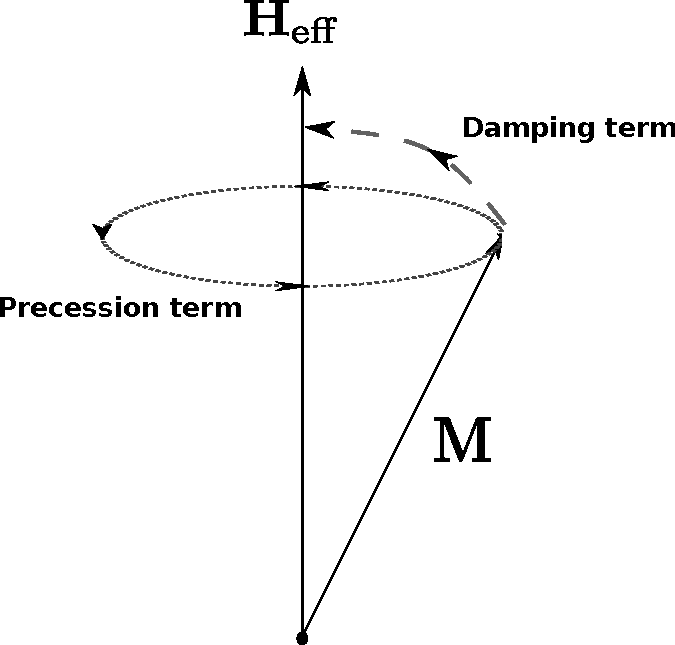
\includegraphics[width=0.6\textwidth]{./images/LLG-terms}
  \caption{The effects of the precession and damping terms in the Landau-Lifshitz and Landau-Lifshitz-Gilbert equations on the magnetisation direction, $\Mv$, of a single magnetic moment with a constant effective field.}
  \label{fig:LLG-terms}
\end{figure}

However, there are still problems with this equation.
For large damping as the damping constant is increased the total speed of the motion increases (since the magnitude of the damping term increases and the precession term remains unchanged) which is physically incorrect \cite{Mallinson1987}.
There is a similar equation introduced by Gilbert \cite{Gilbert2004}, called the Landau-Lifshitz-Gilbert equation, which does not suffer from this problem\footnote{A number of papers give different signs for the LLG equation, this may be due to confusion over the use of $\gamma_L$ to mean $\abs{\gamma_L} = -\gamma_L$. Alternatively it may be due to the lack of specification of the sign of the damping parameter in Gilbert's derivation of the LLG \cite{Gilbert2004} (originally from his thesis), which uses the alternative notation $\alpha = -\eta \abs{\gamma_L} M_s$ where $\eta$ is the usual damping parameter. The correct signs are the ones given here and in reference \cite{Mallinson2000}.}
\begin{equation}
  \label{eq:Gilbert}
  \dMdt = - \gymagc \Mv \times \Hv + \frac{\dampc}{M_s} (\Mv \times \dMdt),
\end{equation}
where $\dampc \neq \dampc_L$. \Cref{eq:Gilbert} can be rearranged into the same form as \cref{eq:LL}, giving
\begin{equation}
  \label{eq:LLG}
  \dMdt = \frac{-\gymagc}{1 + \dampc^2} \Big[ (\MxH) + \frac{\dampc}{M_s} \Big(\Mv \times (\MxH) \Big) \Big],
\end{equation}
which we refer to as the Landau-Lifshitz form of the Landau-Lifshitz-Gilbert equation.

\Cref{eq:LL,eq:Gilbert,eq:LLG} link the unknown magnetisation vector as a function of time, $\Mv(t)$, with the effective field, $\Hv$.
To determine $\Mv$ at an arbitrary time we need to integrate either of the above equations with respect to time starting from a known initial magnetisation $\Mv(0)$.
This is usually done numerically by employing a time integration method, as will be discussed in \cref{sec:time-discretisation}.

Note that there is no spatial dependence directly contained in \cref{eq:LL,eq:Gilbert,eq:LLG}.
However the exchange effective field and magnetostatic field may contain spatial dependence, so usually the final equation to be solved after all substitutions is a partial differential equation (PDE).

% Examples of currently available micromagnetic models include the \oommf \cite{oommf-website} and \nmag \cite{Fischbacher2007} packages, which both use the dynamic method exclusively, along with \magpar \cite{Scholz2003} and \texttt{FEMME} \cite{suessco-website} which can use either dynamic or energy based methods.


\subsection{Boundary conditions}
\label{sec:magn-bound-cond}

By far the most commonly used boundary conditions on the magnetisation $\Mv$ (in dimensional form) are \cite[178, 181]{Aharoni1996}
\begin{equation}
  \label{eq:llg-bc}
  \Mv \times \dMdn = \zerov.
\end{equation}

This condition can be arranged into a simpler form: we first note that for \cref{eq:llg-bc} to hold either $\Mv = \zerov$, $\dMdn = \zerov$, or $\Mv$ is parallel to $\dMdn$.
Clearly $\Mv$ is not the zero vector inside the ferromagnet.
Also we know that the magnetisation length does not change,\footnote{Physically this is part of the definition of the problem. The proof that this fact is embodied in the LLG equation is given in \cref{sec:prop-cont-llg}.} therefore $\pd{\Mv}{\av} \cdot \Mv = 0$ for any direction $\av$ (since the change in magnetisation projected onto the magnetisation direction is the change in magnetisation length). 
Hence $\Mv$ and $\dMdn$ cannot be parallel.
So the final boundary condition is simply
\begin{equation}
  \dMdn = \zerov.
\end{equation}

Alternatively, if the solution is periodic and the domain is ``symmetrical'' ??ds expand, periodic boundary conditions can be used \cite{Jeong2010}.
In this case the value of the magnetisation must be identical on opposite sides of the domain.
The domain of the simulation can then be thought of as infinite.

\subsection{Temperature effects}
\label{sec:temperature-effects}
All equations so far in \thisref{sec:comp-meth} are for the zero temperature case.
Moderate temperature effects (significantly below the Curie temperature) can modelled by adding a stochastic term to the effective field, as done by \eg \cite{DAquino2006}.
High temperature effects require variation of the material parameters with temperature, as well as additional terms to model the dynamic changes of the magnetisation length when near the Curie temperature.
This is typically done by using the Landau-Lifshitz-Bloch equation instead of the Landau-Lifshitz-Gilbert equation, see for example \cite{Evans2012}.
Such models are beyond the scope of this thesis.


\section{Non-dimensionalisation}
\label{sec:normalisations-appendix}

In general it is useful to remove all unnecessary parameters from a differential equation before attempting so solve it.
The main advantage of this is that we simplify the problem and greatly reduce the number of numerical experiments needed to cover all possible situations.
Also for all problems the appropriate discretisation parameters (time step size and mesh size) will be roughly the same. 

\subsection{Non-dimensionalisation of the Landau-Lifshitz-Gilbert equation}
\label{sec:land-lifsh-gilb-normalisation}

We start from the Landau-Lifshitz-Gilbert equation with the magnetostatic, applied, exchange and magnetocrystalline (effective) fields. 
\begin{align}
  \pd{\Mv^*}{t^*} &= - \gymagc \Mv^* \times \Hv^* + \frac{\alpha}{M_s} \Mv^* \times \pd{\Mv^*}{t^*}, 
                    \label{eqn:llgnd} \\
  \Hv^* &= \Happ^* - \nabla^* \phi^* + \frac{2\Exchc^*}{\mu_0 M_s} \nabla^{*2} \mv + \frac{2\Kone^*}{\mu_0 M_s} (\mv \cdot \ev) \ev,
          \label{eqn:effnd} \\
  \nabla^{*2} \phi^* &= \nabla^* \cdot \Mv^*, 
                       \label{eqn:phind}
\end{align}
where we use $^*$ to denote the dimensional variables, operators and constants that will be non-dimensionalised. We assume for simplicity that $M_s$, $\Exchc$ and $\Kone$ are all
constant throughout the magnetic materials used.

Let
\begin{equation}
  \label{eqn:nddefs}
  \begin{aligned}
    \Mv^* &= M_s \mv,  \\
    \phi^* &= \Phi \phi,  \\
    \Hv^* &= M_s \hv,  \\
    \Kone^* &= \nK \kone,  \\
    t^* &= \frac{1}{\gymagc M_s} t,  \\
    x_i^* &= l x_i. 
  \end{aligned}
\end{equation}
Note that $\Mv$ and $\Hv$ have the same units so we use the same normalisation factor. For dimensional purposes derivatives are equivalent to division by the variable differentiated with respect to, so $\nabla^* = \frac{1}{l} \nabla$, $\pd{a}{t^*} = \gymagc M_s \pd{a}{t}$ etc.

Combining \cref{eqn:llgnd} with the definitions~\cref{eqn:nddefs} gives
\begin{equation}
   \dmdt \gymagc M_s^2 =
  - \gymagc M_s^2 \mv \times \hv + \frac{\alpha}{M_s} \gymagc M_s^3 \mv \times \dmdt,
\end{equation}

cancelling the various constants results in the non-dimensionalised Landau-Lifshitz-Gilbert equation
\begin{equation}
  \label{eq:53}
  \dmdt = - (\mv \times \hv) + \alpha (\mv \times \dmdt).
\end{equation}

Similarly for \cref{eqn:phind} we have
\begin{align*}
  \frac{1}{l^2} \Phi \nabla^{2} \phi &= \frac{1}{l} M_s \nabla \cdot \mv, \\
  \frac{\Phi}{M_s l} \nabla^{2} \phi &= \nabla \cdot \mv.
\end{align*}

Letting $\Phi = M_s l$ we obtain
\begin{equation}
  \label{eq:57}
  \lap \phi = \nabla \cdot \mv.
\end{equation}

Repeating the substitutions for \cref{eqn:effnd} gives
\begin{align*}
  M_s \hv &= M_s \happ - \frac{\Phi}{l} \nabla \phi + \frac{2 \Exchc }{\mu_0 M_s} \frac{1}{l^2} \lap \mv + \frac{2\kone}{\mu_0 M_s}  \nK (\mv \cdot \ev) \ev, \\
  \hv &= \frac{M_s}{M_s} \happ - \frac{M_s}{M_s} \nabla \phi + \frac{2 \Exchc}{\mu_0 M_s^2} \frac{1}{l^2} \lap \mv + \frac{2\kone}{\mu_0 M_s^2} \nK (\mv \cdot \ev) \ev, \\
  \hv &= \happ - \nabla \phi + \frac{2 \Exchc}{\mu_0 M_s^2} \frac{1}{l^2} \lap \mv + \frac{2\kone}{\mu_0 M_s^2} \nK (\mv \cdot \ev) \ev, \\
\end{align*}

This can be further simplified by choosing the exchange length\footnote{There are actually two exchange lengths: one based on the strength of exchange as compared with the magnetostatic field and another by comparison with the magnetocrystalline anisotropy. We use the magnetostatic-field-based exchange length for normalisation to avoid division by zero in the case of zero magnetocrystalline anisotropy.} as the characteristic length scale
\begin{equation}
  \label{eqn:l-normalisation}
  l = \sqrt{ \frac{2 \Exchc}{\mu_0 M_s^2} },
\end{equation}

and
\begin{equation}
  \label{k-normalisation}
  \nK = \frac{ \mu_0 M_S^2}{2}.
\end{equation}

So the final system of equations is
\begin{equation}
  \begin{aligned}
    \dmdt &= - \mv \times \hv + \alpha \mv \times \dmdt, \\
    \hv &= \happ - \nabla \phi + \lap \mv + \kone (\mv \cdot \ev) \ev, \\
    \lap \phi &= \nabla \cdot \mv.
    \label{eqn:nd-llg-full}
  \end{aligned}
\end{equation}

From \cref{eq:llg-bc} the dimensional boundary conditions on the LLG with no surface anisotropy are:
\begin{equation}
  \Mv^* \times \pd{\Mv^*}{\nv^*} = 0.
\end{equation}
Using the substitutions from above this becomes
\begin{equation}
  \begin{aligned}
    \frac{M_s^2}{l} \mv \times \dmdn &= \zerov, \\
    \mv \times \dmdn &= \zerov.
  \end{aligned}
\end{equation}

\subsection{Non-dimensionalisation of the Landau-Lifshitz form of the LLG}
\label{sec:land-lifsh-normalisation}

The dimensional Landau-Lifshitz form of the LLG is given in \cref{eq:LLG}:
\begin{equation}
  \label{eq:ll-nd}
  (1 + \dampc^2) \pd{\Mv^*}{t^*} = - \gymagc \Mv^* \times \Hv^*
  - \frac{\gymagc \dampc}{M_s} \Mv^* \times (\Mv^* \times \Hv^*).
\end{equation}
The non-dimensionalisation process is essentially the same as for the Gilbert form, by substituting in the normalisations in \cref{eqn:nddefs} we obtain
\begin{equation}
  (1 + \dampc^2) \dmdt = - \mv \times \hv - \dampc \mv \times (\mv \times \hv).
  \label{eq:ll-nd-llglike}
\end{equation}
The field equations are identical to those in \cref{eqn:nd-llg-full}.


Alternatively the time variable could be normalised differently to remove the factor of $(1 + \dampc^2)$ by using
\begin{equation}
  t^* = \frac{1 + \dampc^2}{\gymagc M_s} t.
\end{equation}
This results in
\begin{equation}
  \dmdt = -\mxh -\dampc \mxmxh.
  \label{eq:ll-nd-simpler}
\end{equation}
However this means that time scale changes (\ie the $t^*$s are different) when switching between the two forms \cref{eq:ll-nd-simpler,eq:53}, making comparisons more difficult.


\subsection{Non-dimensionalisation of the energy}
\label{sec:energy-calculations}

We repeat the process used in \cref{sec:land-lifsh-gilb-normalisation} to get a set of non-dimensionalised energy equations, starting from the equations given in \cref{sec:energy-magnetic-body}:

\begin{equation}
  \Eapp^* = - \mu_0 \int_{\magd} \Mv^* \cdot \Happ^* \d \magd^*,
\end{equation}
\begin{equation}
  \Ems^* =  \frac{-\mu_0}{2} \int_{\magd} \Mv^* \cdot \Hms^* \d \magd^*,
\end{equation}
\begin{equation}
  \Eex^* =  \Exchc \int_{\magd} (\nabla^* \mv)^2 \d \magd^*,
\end{equation}
\begin{equation}
  \Eca^* =  -\Kone^* \int_\magd (\mv \cdot \ev)^2 \d \magd^*.
\end{equation}

We substitute definitions~\cref{eqn:nddefs,eqn:l-normalisation,k-normalisation} and $E^* = \nE e = \mu_0 M_s^2 l^d \, e$ where $d$ denotes the number of spatial dimensions to obtain
\begin{equation}
  \eapp = -\mu_0 M_s^2 l^d \frac{1}{\nE} \int_{\magd} \mv \cdot \happ \d \magd
  = - \int_{\magd} \mv \cdot \happ \d \magd,
  \label{eq:nd-e-app}
\end{equation}
\begin{equation}
  \ems = \frac{-\mu_0 M_s^2 l^d}{2} \frac{1}{\nE} \int_{\magd} \mv \cdot \hms \d \magd
  = -\frac{1}{2} \int_{\magd} \mv \cdot \hms \d \magd,
  \label{eq:nd-e-ms}
\end{equation}
\begin{equation}
  \eex =  \frac{\mu_0 M_s^2 l^2}{2} \frac{l^d}{l^2} \frac{1}{\nE} \int_{\magd} (\nabla \mv)^2 \d \magd
  = \frac{1}{2} \int_{\magd} (\nabla \mv)^2 \d \magd,
  \label{eq:nd-e-ex}
\end{equation}
\begin{equation}
  \eca = - \frac{\mu_0 M_s^2}{2 } l^d \kone \frac{1}{\nE} \int_\magd (\mv \cdot \ev)^2 \d \magd
  = \frac{-\kone}{2} \int_\magd (\mv \cdot \ev)^2 \d \magd.
  \label{eq:nd-e-ca}
\end{equation}
Note that we have used
\begin{equation}
  \d \magd^* = \d (x^*)^d = l^d \d x^d = l^d \d \magd.
\end{equation}


\section{Geometric properties of the continuous Landau-Lifshitz-Gilbert equation}
\label{sec:prop-cont-llg}

The term ``geometric'' properties of a differential equation refers to the properties which do not vary in time \cite[73]{Iserles2009}, \ie conservation laws.
In \thisref{sec:prop-cont-llg} we demonstrate some geometric properties of the Landau-Lifshitz-Gilbert equation.

For this purpose it is convenient to write the non-dimensional LLG equation in the form
\begin{equation}
  \label{eq:llg-prop-form}
  \dmdt = - \mv \times( \hv - \dampc \dmdt),
\end{equation}
where $\hv$ is the effective field including various effects depending on the system being modelled.

We will also need the identity
\begin{equation}
  \label{eq:dot-cross-id}
  \ip{\av}{\av \times \bv} = 0,
\end{equation}
which is true for all inner products $\ip{\cdot}{\cdot}$ because $\av \times \bv$ is perpendicular to $\av$ by the definition of the cross product.
In particular, it is true for the dot product of two vectors (also known as scalar multiplication) and the $\ltwo$ inner product.

We first show that length of the magnetisation at any point is constant over time.
To see this we take the dot product of~\cref{eq:llg-prop-form} with $\mv$ and use~\cref{eq:dot-cross-id} to obtain
\begin{equation}
  \label{eq:56}
  \mv \cdot \dmdt = 0.
\end{equation}
This equation implies that the change of $\mv$ over time is always perpendicular to $\mv$, so length is conserved.\footnote{Actually this is obvious from the fact that $\dmdt$ is can be written as a cross product involving $\mv$, but the technique used here is useful in the discussion of the properties of various discrete forms of the Landau-Lifshitz-Gilbert equation.}

Next we look at the energy properties of the system described by the Landau-Lifshitz-Gilbert equation.
The change in energy over time can be derived similarly to the change in magnetisation by taking the $\ltwo$ inner product\footnote{The $\ltwo$ inner product is given by $\ltip{\av}{\bv} = \int_\magd \av \cdot \bv \d\magd$.} of each side of~\cref{eq:llg-prop-form} with $\hv - \dampc \dmdt$.
We then use the identity~\cref{eq:dot-cross-id} to find that
\begin{equation}
  \label{eq:58}
  \ltip{\hv}{\dmdt} - \dampc \ltip{\dmdt}{\dmdt} = 0.
\end{equation}
Using the fact that $\hv = -\vd{\e}{\mv}$ and the chain rule for variational derivatives, we find that the time derivative of the energy is given by
\begin{align*}
  \pd{\e[\mv(\xv, t), t]}{t} &= \ltip{\vd{e}{\mv}}{\dmdt} - \ltip{\pd{\happ}{t}}{\mv} \\
                             &= -\ltip{\hv}{\dmdt} - \ltip{\pd{\happ}{t}}{\mv},
\end{align*}
and so
\begin{equation}
  \ltip{\hv}{\dmdt} = -\pd{\e}{t} - \ltip{\pd{\happ}{t}}{\mv}.
  \label{eq:64}
\end{equation}
Finally, substituting \cref{eq:64} into \cref{eq:58} leaves
\begin{equation}
  \label{eq:energy-decay}
  \pd{\e}{t} = -\dampc \ltip{\dmdt}{\dmdt} - \ltip{\pd{\happ}{t}}{\mv}.
\end{equation}
\Cref{eq:energy-decay} shows that under constant applied field the energy of the system is always decreasing at a rate proportional to $\dampc$.
For non-constant applied fields the change in the Zeeman energy can increase or decrease the energy depending on how the field is changed. % field moves towards m - decrease, away -> increase. For non-spatially constant this is averaged over space in some sense by the inner product.
In fact, the first term of \cref{eq:energy-decay} can be easily derived from the Rayleigh dissipation functional used as the basis for the derivation of the Gilbert form of the LLG \cite{Gilbert2004}.

Note that length conservation is a \emph{point-wise} property, \ie $\abs{\mv} = 1$ at every point in space. 
In contrast the energy decay/conservation is a \emph{global} property, \ie an integral over all space is conserved.
This is related to the use of the dot product and the $\ltwo$ inner product respectively in the derivations above.


%%% Local Variables:
%%% mode: latex
%%% TeX-master: "./main"
%%% End:
